\begin{lstlisting}[style=base]
def psychofun_vec(theta,stim):
    """Psychometric function vectorized"""
    @mu = theta[:,0]@           # bias
    @sigma = theta[:,1]@        # slope
    @lapse = theta[:,2]@         # lapse rate
    @lapse_bias = theta[:,3]@    # lapse bias}
    p_right = norm.cdf(stim,loc=mu,scale=sigma)    
    p_right = lapse*lapse_bias + (1-lapse)*p_right # Adding lapses
    return p_right

def psychofun_timevarying_loglike_vec(theta,df):
    """Log-likelihood for time-varying model"""
    s_vec = np.array(df['signed_contrast']) # Stimulus values
    r_vec = np.array(df['response_choice'])  # Responses
    Ntrials = len(s_vec)
    mu = np.linspace(theta[0],theta[4],Ntrials)
    sigma = np.linspace(theta[1],theta[5],Ntrials)
    lapseR = np.linspace(theta[2],theta[6],Ntrials)
    lapseB = np.linspace(theta[3],theta[7],Ntrials)
    @ThetaMat = np.transpose(np.asarray([mu,sigma,lapseR,lapseB]))@ 
    @p_right = psychofun_vec(ThetaMat,s_vec)@
    loglike = np.sum(np.log(p_right[r_vec == 1])) + np.sum(np.log(1 - p_right[r_vec == -1]))
    return loglike
\end{lstlisting}

\begin{figure}[!hbt]
\begin{center}
 \makebox[\textwidth]{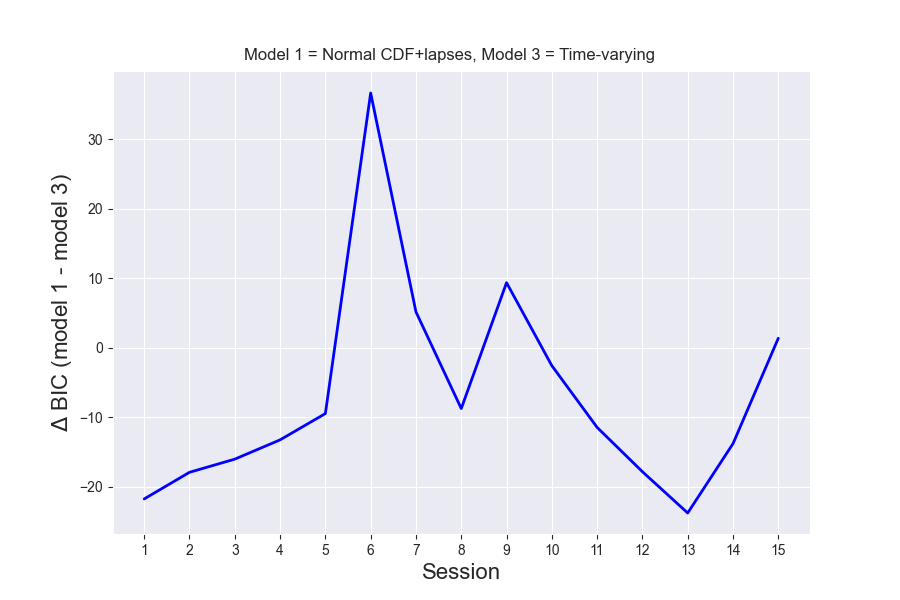
\includegraphics[width=10  cm]{BIC_time-varying.png}}
\end{center}
\caption{Differences between the 3 models ($\Delta$ BIC). A positive value shows stronger evidence for the Model 3 relatively to Model 1 (left) or Model 2 (right).}
\label{fig:time}
\end{figure}